
\begin{listing*}[]
\begin{minipage}{.35\textwidth}
\begin{minted}
[
fontsize=\footnotesize,
linenos=true,
escapeinside=||,
breaklines
]
{go}
package main
import "sync"

type Container struct{ |\label{bugListing:containerType_start}|
  sync.Mutex
  stop  chan struct{}
} |\label{bugListing:containerType_end}|

func main() {
  container := &Container{ |\label{bugListing:container_create_start}|
       stop:make(chan struct{})} |\label{bugListing:container_create_end}|
  go Monitor(container) |\label{bugListing:main_go_monitor}|
  go StatusChange(container) |\label{bugListing:main_go_statChange}|
}
\end{minted}
\end{minipage}
\begin{minipage}{.35\textwidth}
\begin{minted}
[
fontsize=\scriptsize,
linenos=true,
escapeinside=||,
breaklines
]
{go}
|\setcounter{FancyVerbLine}{15}|func Monitor(cnt *Container){
  for{
    select{|\label{bugListing:Monitor_select}|
    case <- cnt.stop:  |\label{bugListing:Monitor_case_recv}|
      return |\label{bugListing:Monitor_case_recv_ret}|
    default: |\label{bugListing:Monitor_case_def}|
      cnt.Lock()  |\label{bugListing:Monitor_case_def_lock}|
      cnt.Unlock() |\label{bugListing:Monitor_case_def_unlock}|
}}}
func StatusChange(cnt *Container){
  cnt.Lock() |\label{bugListing:statChange_lock}|
  defer cnt.Unlock() |\label{bugListing:statChange_defer_unlock}|
  cnt.stop <- struct{}{} |\label{bugListing:statChange_send}|
}
\end{minted}
\end{minipage}
\begin{minipage}{.25\textwidth}
  \centering
  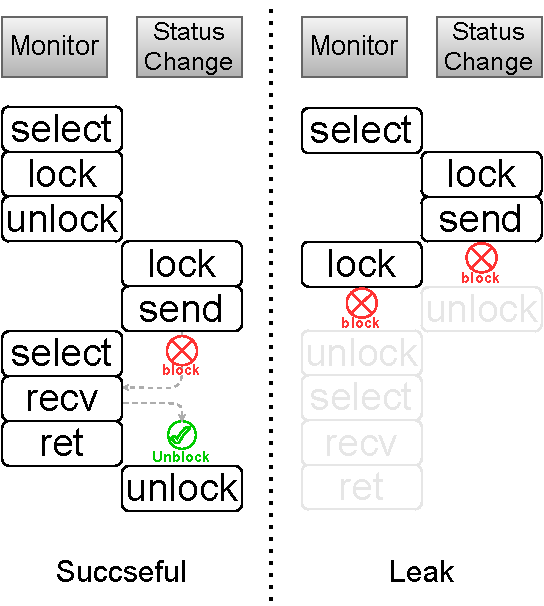
\includegraphics[width=.99\linewidth]{figs/execViz_moby.pdf}
\end{minipage}
\caption{Simplified version of bug \texttt{moby28462}}
\label{listing:moby28462.minipage}
\end{listing*}

%\begin{listing}[]
\begin{minipage}{.45\columnwidth}
\begin{minted}
[
fontsize=\footnotesize,
linenos=true,
escapeinside=||,
xleftmargin=2em,
breaklines
]
{go}
package main
import "sync"

type Cont struct{|\label{bugListing:containerType_start}|
  sync.Mutex
  stop  chan struct{}
}|\label{bugListing:containerType_end}|

func main() {
  cnt := &Cont{|\label{bugListing:container_create_start}|
       stop:make(chan struct{})}|\label{bugListing:container_create_end}|
  go Monitor(cnt)|\label{bugListing:main_go_monitor}|
  go StatusChange(cnt)|\label{bugListing:main_go_statChange}|
}
\end{minted}
\end{minipage}\hfill
\begin{minipage}{.45\columnwidth}
\begin{minted}
[
fontsize=\footnotesize,
linenos=true,
escapeinside=||,
breaklines
]
{go}
|\setcounter{FancyVerbLine}{15}|func Monitor(cnt *Cont){
  for{
    select{
    case <- cnt.stop:  |\label{bugListing:Monitor_case_recv}|
      return |\label{bugListing:Monitor_case_recv_ret}|
    default: |\label{bugListing:Monitor_case_def}|
      cnt.Lock()  |\label{bugListing:Monitor_case_def_lock}|
      cnt.Unlock() |\label{bugListing:Monitor_case_def_unlock}|
}}}
func StatusChange(cnt *Cont){
  cnt.Lock() |\label{bugListing:statChange_lock}|
  defer cnt.Unlock() |\label{bugListing:statChange_defer_unlock}|
  cnt.stop <- struct{}{} |\label{bugListing:statChange_send}|
}
\end{minted}
\end{minipage}
\caption{Simplified version of bug \texttt{moby28462}}
\label{listing:moby28462}
\end{listing}


\subsection{Go Concurrency}
\label{sec:goConcurrency}
%
Go introduces a new concurrency model, mixing shared-memory features of languages like Java/C/C++ and message-passing concepts such as Erlang's, with an ad-hoc scheduler that orchestrates Go's concurrent components interactions while shielding the user from many low-level aspects of the runtime.
%
The language is equipped with a rich vocabulary of \textit{serialization} features to facilitate the memory model constraints~\cite{go-memModel}; they include synchronous and asynchronous communication, memory protection, and barriers for efficient synchronization:
\begin{itemize}
    \item \textbf{Goroutines} are functions that execute concurrently on logical processors.
    \item \textbf{Channels} are typed conduits through which goroutines communicate.  Channels are unbuffered by default, providing synchronous (rendezvous) or asynchronous (via buffered channels) messaging between goroutines.
    \item \textbf{Synchronization} features such as \textit{(RW)mutex}, \textit{waitGroup}, \textit{conditional variables}, and \textit{select} are included in the language to provide more and flexible synchronization, data access serialization, and memory protection.
    \item \textbf{Scheduler} maintains goroutines in FIFO queues and binds them on OS threads to execute on processing cores.
\end{itemize}


This design facilitates the construction of data flow models that efficiently utilize multiple CPU cores and encourages developers to \textit{share memory through communication} for safe and straightforward concurrency and parallelism.
%
This rich mixture of features has, unfortunately, greatly exacerbated the complexity of debugging.
%
In fact, the popularity of Go has outpaced its debugging support~\cite{go-survey,tu-concurrentBugs-asplos19,yuan-gobench-cgo21}.
%
There are some encouraging developments in support of debugging, such as a data race checker \cite{go-race-blog} that has now become a standard feature of Go and has helped catch many a bug.
%
However, the support for blocking bugs such as deadlocks and Go-specific bug-hunting support for Go idioms (e.g., misuse of channels and locks) remain insufficiently addressed.



%\begin{listing}[]
\begin{minipage}{.5\textwidth}
\begin{minted}
[
fontsize=\scriptsize,
linenos=true,
escapeinside=||,
breaklines
]
{go}
package main
import "sync"

type Container struct{ |\label{bugListing:containerType_start}|
  sync.Mutex
  stop  chan struct{}
} |\label{bugListing:containerType_end}|

func main() {
  container := &Container{ |\label{bugListing:container_create_start}|
       stop:make(chan struct{})} |\label{bugListing:container_create_end}|
  go Monitor(container) |\label{bugListing:main_go_monitor}|
  go StatusChange(container) |\label{bugListing:main_go_statChange}|
}
\end{minted}
\end{minipage}
\begin{minipage}{.35\textwidth}
\begin{minted}
[
fontsize=\scriptsize,
linenos=true,
escapeinside=||,
breaklines
]
{go}
|\setcounter{FancyVerbLine}{15}|func Monitor(cnt *Container){
  for{
    select{
    case <- cnt.stop:  |\label{bugListing:Monitor_case_recv}|
      return |\label{bugListing:Monitor_case_recv_ret}|
    default: |\label{bugListing:Monitor_case_def}|
      cnt.Lock()  |\label{bugListing:Monitor_case_def_lock}|
      cnt.Unlock() |\label{bugListing:Monitor_case_def_unlock}|
}}}
func StatusChange(cnt *Container){
  cnt.Lock() |\label{bugListing:statChange_lock}|
  cnt.stop <- struct{}{} |\label{bugListing:statChange_send}|
  cnt.Unlock() |\label{bugListing:statChange_defer_unlock}|
}
\end{minted}
\end{minipage}
\begin{minipage}{.29\textwidth}
  \centering
  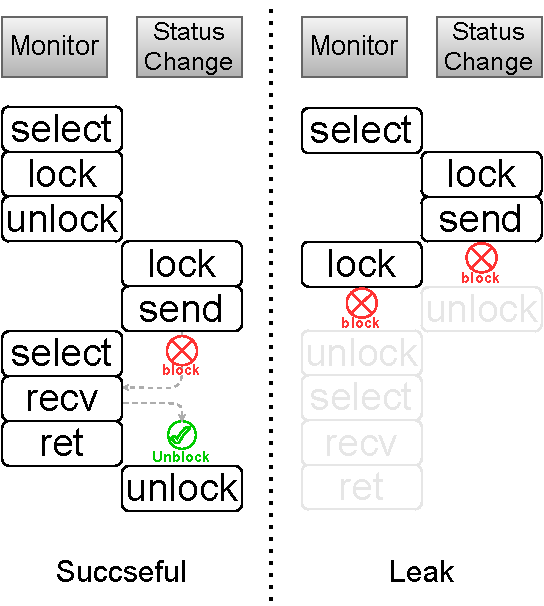
\includegraphics[width=.99\linewidth]{figs/execViz_moby.pdf}
\end{minipage}
\caption{Simplified version of bug \texttt{moby28462}}
\label{listing:moby28462}
\end{listing}


%\stcmtside{Explaining the example to motivate}
Listing \ref{listing:moby28462.minipage} shows a simplified version of a reported bug in Docker \cite{moby-28462-commit}.
%
An instance of the \texttt{Container} type (lines \ref{bugListing:containerType_start}-\ref{bugListing:containerType_end}) is created in the \texttt{main} function (lines \ref{bugListing:container_create_start}-\ref{bugListing:container_create_end}).
%
In line \ref{bugListing:main_go_monitor}, a goroutine is spawned to execute function \texttt{Monitor} that continuously checks the container status and returns once it receives from the container's channel (lines \ref{bugListing:Monitor_case_recv}-\ref{bugListing:Monitor_case_recv_ret}).
%
The default case of the \texttt{select} statement (line \ref{bugListing:Monitor_case_def}) allows \texttt{Monitor} to continue monitoring without getting blocked on the channel receive (line \ref{bugListing:Monitor_case_recv}).
%
Concurrent to the \texttt{main} and \texttt{Monitor} goroutines, another goroutine is created in line  \ref{bugListing:main_go_statChange} to execute function \texttt{StatusChange} which changes the status of the container by sending to the container's channel.
%
The container's lock is released after the send action completes and function returns (\texttt{defer} statement in line \ref{bugListing:statChange_defer_unlock}).
%


Native execution of this program terminates successfully without issuing any error or warning.
%
Based on the Go specification and memory model, there is no constraint on the goroutines spawned from the \texttt{main} function to join back before the \texttt{main} goroutine\footnote{In the remainder of the paper, we use \textit{main function} and \textit{main goroutine} interchangeably.} terminates.
%
A deadlock detector within the runtime periodically checks that the scheduler queues of all \textit{runnable} goroutines never become empty until the \texttt{main} goroutine terminates.
%
In other words, the runtime throws a deadlock exception when the \texttt{main} goroutine is blocked, and no other goroutine is in the queue to execute (\ie, \textit{global deadlock}).
%
Since there is no blocking instruction in the \texttt{main} goroutine in listing \ref{listing:moby28462.minipage}, the program terminates successfully regardless of other goroutines' statuses.
%
However, this program suffers from a common bug in concurrent Go where one or more goroutines \textit{leak} (\ie, \textit{partial deadlock}) from the execution (\ie, never reach their end states).

%\stcmtside{Explain the deadlock (leak) situation that might get overlooked}
%Due to the non-determinism introduced by the runtime scheduler and application-level random features like \texttt{select}, many interleavings are feasible for concurrent execution of simple programs such as listing \ref{listing:moby28462.minipage}.
%
The right side of the listing displays a successful run and a leak situation of the program.
%
In the leak situation, first, the \texttt{Monitor} goroutine executes the \texttt{select} statement and, based on the available cases, picks the default case to execute.
%
Right before the execution of mutex lock (line \ref{bugListing:Monitor_case_def_lock}), the scheduler context-switches and the \texttt{StatusChange} goroutine starts its execution through which it holds the lock and blocks on sending to the channel (line \ref{bugListing:statChange_send}) since there is no receiver on that channel.
%
Upon blocking on send, the scheduler transfers back the control to the \texttt{Monitor} goroutine that tends to acquire the mutex, but because the mutex is already held by \texttt{StatusChange}, the \texttt{Monitor} goroutine also blocks.
%
The circular wait between the container mutex and channel prevents both spawned goroutines from reaching their end states and leaves the program in an unnoticed deadlock situation.
%
%\stcmtside{The thirst for novel and scalable debuggers}
%Widely used deadlock detectors such as Goodlock \cite{havelund-goodlock-spin00} are not applicable in Go since causes of Go deadlocks are resources (\eg, locking a locked mutex) or communication (\eg, sending on a full channel), or a combination of them (\eg, leaky interleaving of listing \ref{listing:moby28462.minipage}).
%
%In addition, due to the lightweight nature of goroutines, it is not uncommon to spawn thousands of goroutines in production software systems.
%
%Hence,  novel and scalable techniques are needed to enable realistic modeling of program behavior during execution.
%

\subsection{Concurrency Bugs in Go}
\label{sec:goBugs}
Based on a proposed bug taxonomy for Go \cite{tu-concurrentBugs-asplos19}, bugs are categorized separately based on their \textit{causes} (shared-memory vs. message-passing) and \textit{symptoms} (blocking vs. non-blocking).
%
Blocking bugs historically refer to situations where one or more processing units (\eg, goroutines) are blocked, waiting for an external signal to resume (\eg, leak situation in listing \ref{listing:moby28462.minipage}.
%
The observed causes of such blocking flaws in the context of Go are as follows:

\begin{itemize}
  \item \textit{Resource deadlocks}: Go inherits resource deadlocks from multithreaded languages like Java and C/Pthreads where goroutines are trapped in a circular wait for the resource (\eg, mutex) that is held by other goroutines.
  \item \textit{Communication deadlocks}: Synchronized (unbuffered) channels transmit values from one goroutine to another in a rendezvous fashion. The sender (receiver) blocks until the receiver (sender) is ready to receive (send). Misuse of channel operations might result in one or more goroutines waiting for a sender/receiver to unblock them forever.
  \item \textit{Mixed deadlocks}: The leak situation in listing \ref{listing:moby28462.minipage} is the example of such deadlocks where one goroutine is blocked on acquiring a resource that is held by another goroutine which is blocked on communication.
\end{itemize}

Similar to other concurrent languages, Go has non-blocking bugs such as data races and atomicity violations while introducing new bug idioms due to its new concepts such as anonymous functions \cite{tu-concurrentBugs-asplos19}.
%
This work focuses on blocking bugs (i.e., partial and global deadlocks).

%\stcmt{below: Application-level non-determinism makes debugging more difficult}
%\noindent{\bf Application-level non-determinism:\/}
In addition to the non-deterministic nature of concurrent languages caused by the scheduler and interaction between concurrent components, Go introduces some level of non-determinism at the application level.
%
The \textit{select-case} statement (similar to switch-case) allows the goroutine to wait on multiple channel operations.
%
The runtime picks one case pseudo-randomly among available cases (\ie, channel sends and receives that are ready to execute without blocking).
%
If none of the cases are ready, the executing goroutine is blocked unless there is a \textit{default} case.
%
The default case makes the select non-blocking and prevents the goroutine from waiting for unavailable communications.
%
Such random behavior expands the interleaving space, and it grows exponentially when nested selects are employed in conjunction with nested loops.
%
As a result, tracing the cause of a program's misbehaved execution becomes increasingly tricky.
%
Our observations (section \ref{sec:evaluation}) demonstrate that \textbf{select statements are involved at the center of many rare bugs}.


\subsection{Accelerating Bug Exposure}
Blocking bugs are primarily caused by the non-deterministic decisions that the scheduler makes.
%
Such bugs may not manifest themselves in conventional testing and are difficult to reproduce.
%
Figure \ref{fig:rare_bugs} displays the histogram of 68 blocking bug kernels grouped by the number of trials that \goat takes to detect them.
%
Approximately 30\% of bugs required more than one execution to happen and be detected by \goat\footnote{The figure and numbers are obtained from trials of \goat on native execution of bug kernels without any randomization (\ie, $D=0$).}.
%
\textit{Stress testing} is a common way to detect such rare bugs by exercising the scheduler and examine the program's behavior in many executions.
%
However, such testing is inefficient because some interleavings might get tested repeatedly while other feasible interleavings remain untested.
%
It has been empirically demonstrated that a small amount of randomness in each test execution can drastically reduce the number of iterations needed to find concurrency bugs \cite{thomson-concurrencyTesting-ppopp14,emmi-delayBounded-popl11}.
%
For instance, forcing context-switches before synchronization/serialization operations in concurrent programs increases the probability of finding rare concurrent bugs \cite{burckhardt-depthBug-asplos10}.
%
In listing \ref{listing:moby28462.minipage}, a rare context-switch after the \texttt{select} statement in line \ref{bugListing:Monitor_select} causes the lock operation on mutex $m$ in line \ref{bugListing:Monitor_case_def_lock} of goroutine \texttt{Monitor} to \textit{block} goroutine \texttt{StatusChange} on locking $m$ in line \ref{bugListing:statChange_lock} and causing a deadlock.
%
Concurrency primitive usages (\eg, channel send/recv, mutex lock/unlock, select) are the \textit{critical points} in the program because their behavior directly impacts the blocking behavior of Go programs.
%
In \goat, we statically identify such critical points and inject \textit{yield} handlers before each concurrency primitive usage.
%
During execution, the handlers randomly decide if the current goroutine should yield to other goroutines to execute.
%
Results in section \ref{sec:evaluation} show that such simple yields are effective in detecting rare bugs.

\subsection{Testing Coverage Analysis}
\label{sec:coverage}
To demonstrate that testing has been thorough, \textit{coverage metrics} are defined to measure the progress of tests and specify testing termination conditions.
%
Coverage metric for the set of testing executions $\mathcal{T}$ is a set of \textit{requirements} $\mathcal{R}$ that should get covered during testing iterations.
%
We say requirement $R_i \in \mathcal{R}$ is covered during testing iteration $t_j \in \mathcal{T}$ if we can correlate an \textit{action} during execution of $t_j$ to $R_i$.
%
For example, in \textit{statement coverage}, which is a widely-used metric in testing sequential software, $R$ is the set of source locations (file and line numbers) in the target program.
%
$R_i$ is covered by test execution $t$ if the statement at location $R_i$ is executed in $t$.
%
The \textit{coverage percentage} of a test $\mathcal{T}$ is the ratio of the requirements covered by at least one execution over the number of all requirements ($|R|$).

In the context of concurrent software testing, coverage metrics are proposed to quantify the quality of search space exploration.
%
\textit{Synchronization} coverage metrics such as \textit{blocking-blocked} \cite{edelstein2003contest}, \textit{blocked-pair-follows} \cite{trainin-followsCoverage-padtad09} and \textit{synchronization-pair} \cite{hong-syncTesting-issta12} defined requirements to cover during testing for exposing blocking bugs (\eg deadlocks).
%
%\textit{Memory access} coverage metrics such as PSet \cite{yu-pser-isca09} and def-use \cite{yang-defuse-issta98} focuses on data-access related bugs such as atomicity violation or data races.
%
For example, the synchronization coverage model in \cite{edelstein2003contest} defines \textit{blocking} and \textit{blocked} requirements per each synchronized block (\ie mutually exclusive section of the code that is protected by a lock).
%
The purpose of this requirement is to check if a test can report when there is a lock contention for two or more threads entering the synchronized block.
%
That is, a thread is either \textit{blocked} from entering the synchronization block or \textit{blocking} other threads from entering by holding the lock.
%



\begin{figure}[]
\centering
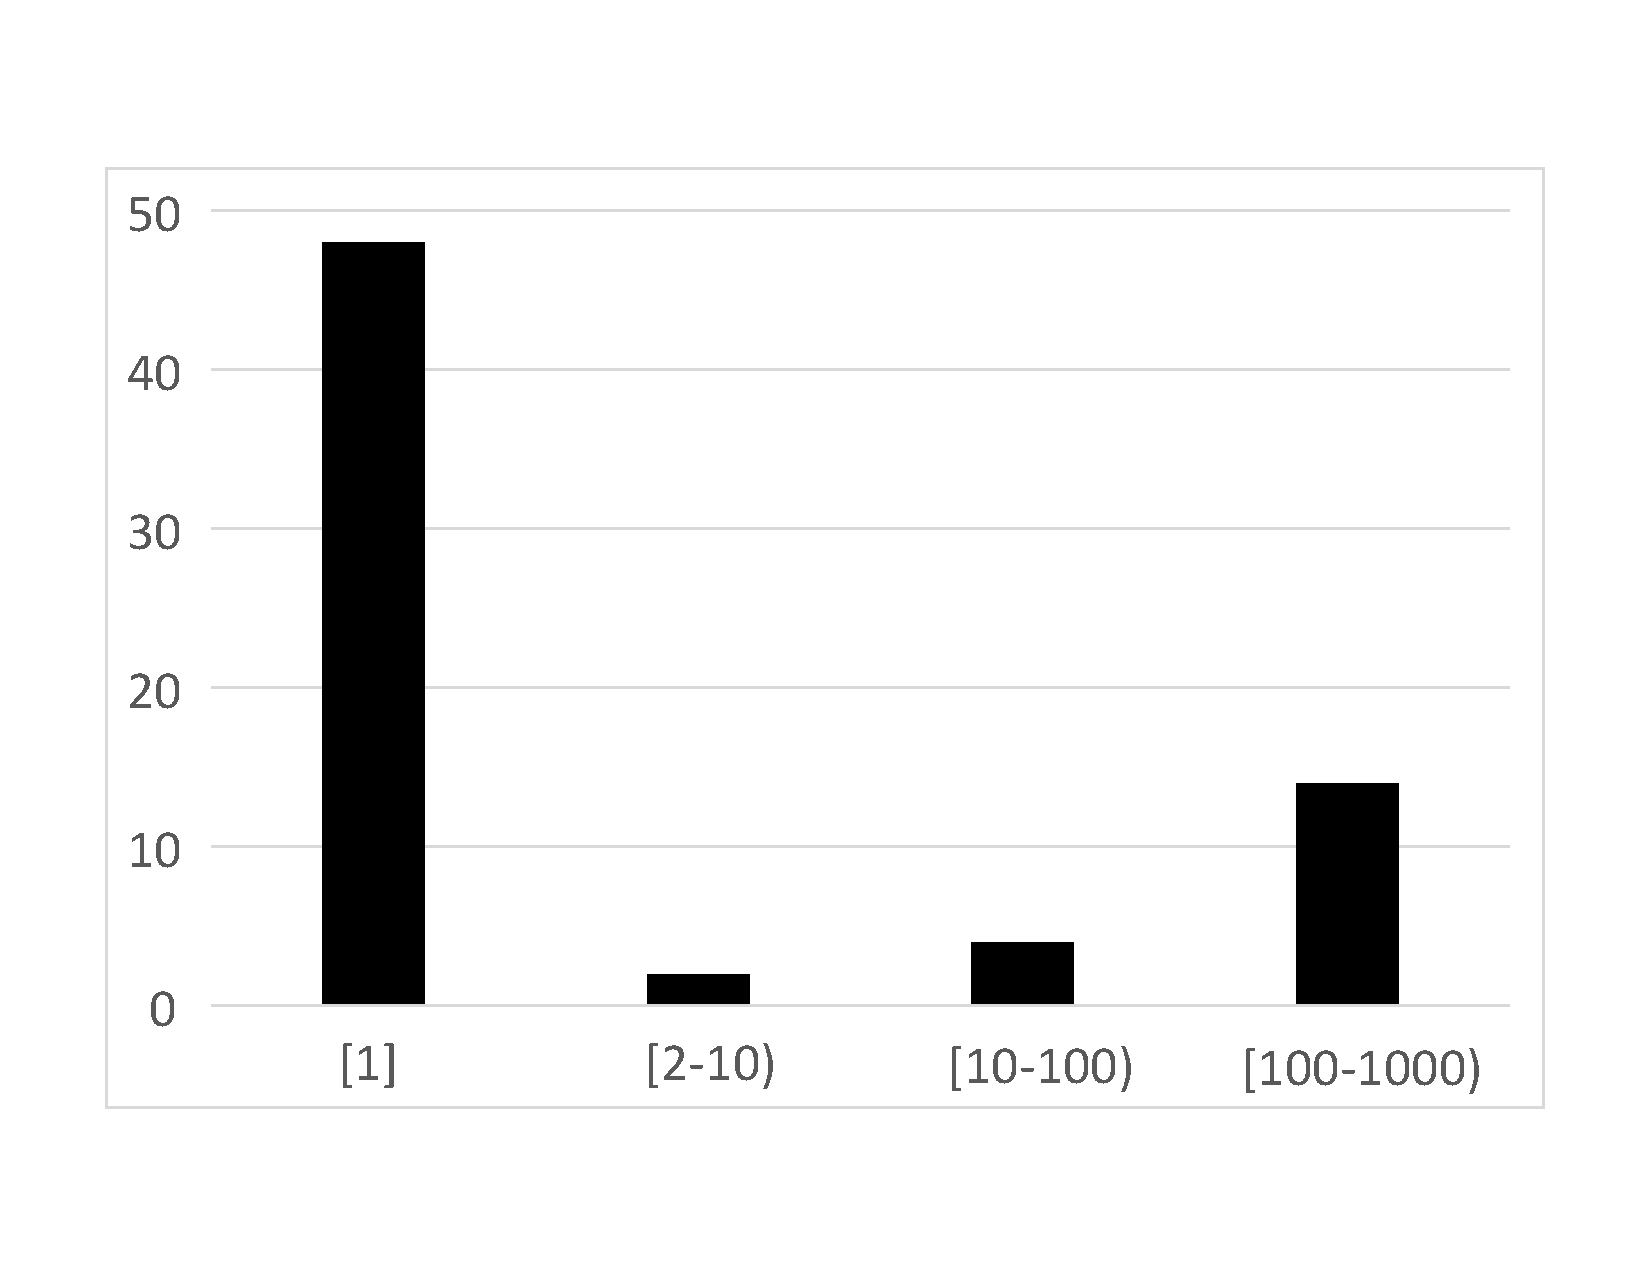
\includegraphics[width=0.7\linewidth]{figs/coverage_motivation.pdf}
%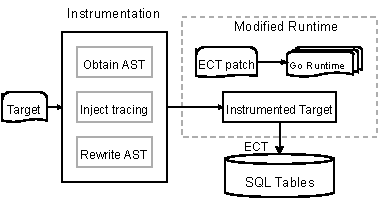
\includegraphics[]{figs/overview.png}
%\includegraphics[]{figs/overv}
\caption{Distribution of number of trials falling into given intervals to detect 68 blocking bugs in GoKer~\cite{yuan-gobench-cgo21} using \goat ($D0$)}
\label{fig:rare_bugs}
\end{figure}


The existing concurrency coverage metrics are primarily in the context of Java and C/Pthreads.
%
They are not necessarily applicable to languages like Go, as such languages have different concurrency primitives and semantics.
%
Novel coverage metrics are required to enable the quantification of interleaving space exploration.
%
Bron et al.,\cite{bron-appSyncCov-ppopp05} enumerates four major characteristics for coverage metrics to gain acceptance:
\begin{enumerate}
  \item \textbf{Static model:} A static model of requirements from the given program should be constructed by instrumenting the source code. The model should be well-understood by the developer or tester before execution. The model should maintain covered requirements during testing executions.
  \item \textbf{Coverable and measurable requirements:} The absolute majority of requirements should be realistic enough to be \textit{coverable} during testing. For a few that are not coverable (due to program semantics) or not \textit{measurable} (because of technical limitations), the developer should be aware of the reason.
  \item \textbf{Actions for uncovered requirements:} After testing terminates, every uncovered requirement should yield an action (\eg, extending testing iterations or removing dead code from the program, thus removing uncoverable requirements)
  \item \textbf{Coverage satisfaction:} Some action should be taken upon reaching a threshold of coverage percentage (e.g., testing phase termination when reaching 100\% statement coverage)
\end{enumerate}

Defining a new coverage metric to satisfy the above characteristics requires an accurate and proper mental model of target bugs.
%
Using the \goat's infrastructure, we studied the underlying causes of many bugs, including GoKer benchmark~\cite{yuan-gobench-cgo21} and propose a set of coverage requirements that enables extensive analysis of dynamic behavior of concurrency primitives under various scheduling scenarios.
%
In section \ref{sec:covreq}, we describe our proposed coverage metric for testing concurrent Go, which is extensible to all concurrent languages.
